%sparsemul_result


Versuch der Vergleichung von matlab,CPU-und GPU-Implimentierung wird in Abb.\ref{sparse_ergebnis}. ausgewiesen. Für 128-Diagonalmatix kann CUDA-Implementierung gegen CPU zu Faktor 9 erreichen.


\begin{figure}[htbp]
%\centering
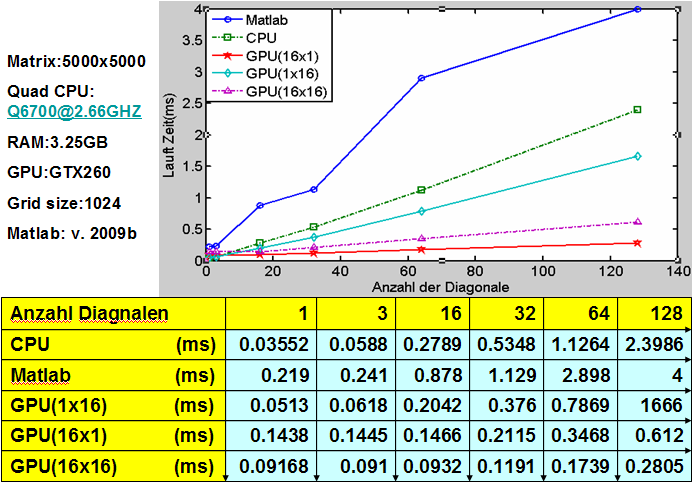
\includegraphics[width=3.5in]{../xby/pic//sparse_ergebnis}
\caption{Vergleichung der sparser Matrizemultiplikation von matlab, CPU-und GPU-Implementierung.}
\label{sparse_ergebnis}
\end{figure}


\begin{table}
%\begin{tabular}{|l|c|c|c|c|c|}
\caption{Ausführungszeiten der Sparse-Matrixmultiplikation} 
\label{sparse_result}
\centering
\begin{tabular}{|p{46pt}p{20pt}p{20pt}p{20pt}p{20pt}p{20pt}p{20pt}|}
%\begin{tabularx}{350pt}{1xxxxx}
\toprule
%\hline
Anzahl Diagonalen& 1& 3& 16& 32& 64 &128\\

\midrule
%\hline
Matlab(ms)&			0.219&   0.241&   0.878&   1.129&   2.898& 4\\
CPU(ms)& 			0.03552&   0.0588& 	0.2789& 0.5348&  1.1264& 2.3986\\
GPU(1x16)(ms)& 0.0513&   0.0618&  0.2042&  0.376&  0.7869& 1.666\\
GPU(16x1)(ms)& 0.1438&	 0.1445&	0.1466&	0.2115&	 0.3468&	0.612\\

GPU(16x16) & 0.09168&	0.091&	0.0932&	0.1191&	0.1739&	0.2805\\
\bottomrule
%\hline     
\end{tabular}
%\end{tabularx}
\end{table}